\chapter{Alcuni richiami di relatività galileiana}

La fisica classica pre-relativistica postulava l'esistenza di spazio e tempo assoluti, che avevano cioè valore indipendentemente 
dal sistema di riferimento utilizzato e che si basavano sulla misurazione di spazi e tempi\footnote{sarebbe più preciso dire lunghezze,
ovvero distanze tra due punti e intervalli temporali, ovvero durate.} uguali in qualunque sistema di riferimento.
In particolare, sia la teoria della relatività galileiana, sia la più completa teoria dinamica di Newton prevedevano 
l'esistenza di un sistema di riferimento inerziale al quale potevano essere ricondotti tutti gli altri attraverso 
le trasformazioni di Galileo. Tale sistema era solitamente identificato con quello delle stelle fisse.

In base a questi principi, qualunque osservazione compiuta in un sistema di riferimento inerziale conserva la misura delle lunghezze 
(per esempio di un regolo) così come gli intervalli di tempo (tra due eventi, come per esempio l'accensione di due lampadine). 
Allo stesso modo, in meccanica classica, due eventi simultanei in un sistema di riferimento (cioè con la stessa coordinata temporale) 
lo sono in ogni sistema di riferimento inerziale. Questo fatto trova il suo riscontro nelle trasformazioni galileiane, rispetto 
alle quali le leggi di Newton presentano una invarianza in forma.

\section{L'osservatore in relatività galileiana}

La concezione newtoniana di osservatore è basata sulla nozione di corpo
rigido (tipica nozione della geometria euclidea proveniente dalla fisica terrestre). 
Inizialmente un osservatore newtoniano è una piccola piattaforma
rigida, che costituisce il supporto dell’osservatore e che definisce il concetto
di localizzazione, nel senso che un evento avviene in un punto di tale piattaforma. 
In ogni punto della piattaforma è situato un orologio in quiete. In
breve, si dice che un osservatore newtoniano è una rete di orologi posti ai
vertici di un reticolato di regoli rigidi.

\begin{figure}[htbp]
  \centering
  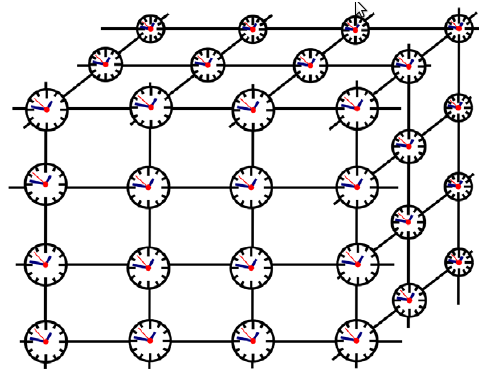
\includegraphics[scale=0.5]{immagini/galileo/oss_newton}
  \caption{Un osservatore come un reticolo di regoli e orologi.}
\end{figure}

In questa definizione si ammette tacitamente (e dal punto di vista matematico questa 
è un’ipotesi topologica sulla struttura dello spaziotempo) che tale reticolato possa 
essere esteso indefinitamente in tutte le direzioni (per questo si parla di coordinate globali), 
e che per le misure spaziali tra punti in quiete rispetto ai reticolati valgano le regole della geometria euclidea.

Per completare la definizione dell’osservatore newtoniano, bisogna infine
sincronizzare gli orologi posti nei diversi punti del reticolato: possiamo pensare 
che ogni punto abbia un suo piccolo ``laboratorio'', e bisogna fare in
modo che tutti questi ``laboratori'' siano sincronizzati. 
Il processo di sincronizzazione può essere fatto, ad esempio, per trasporto di un orologio campione,
e qui ipotizziamo tacitamente che la sincronizzazione non dipenda dal
trasporto e che orologi sincronizzati rimangano sincronizzati.

Il processo di sincronizzazione definisce il concetto di tempo relativo
all’osservatore, definito come il tempo misurato dall’orologio - in quiete
(rispetto alla piattaforma dell’osservatore) e sincronizzato nella rete di orologi
- nel punto in cui avviene l’evento. E chiaro che questa nozione ha significato
solo se gli orologi sono stati precedentemente sincronizzati.

\subsection{Gli assiomi della relaitività galileiana}

Definito il singolo osservatore come un sistema di coordinate globali sullo
spaziotempo (dove l’aggettivo ``globali'' rende conto del fatto che ogni evento
pu` essere localizzato poiché la piattaforma è estendibile all’infinito), rimane
da fare il confronto tra i diversi osservatori, il che equivale a porsi il problema
di un cambio di coordinate sullo spaziotempo.

Nella Relatività newtoniana si ammettono due assiomi, detti del tempo 
assoluto e dello spazio assoluto (in quest’ordine).

\subsubsection{L'assioma del tempo assoluto}
L'assioma del tempo assoluto afferma il carattere invariantivo delle durate, cioè delle differenze di tempo:
gli intervalli temporali tra due eventi misurati da due diversi osservatori newtoniani in moto relativo 
coincidono sempre, indipendentemente dalla natura del moto relativo questo vale, ad esempio, anche per moti non inerziali. 

In particolare, eventi simultanei in un riferimento sono simultanei in ogni altro
riferimento: il concetto di simultaneità è dunque un concetto assoluto, nel senso che è una ``proprietà
 che non dipende dall'osservatore - infatti la Relatività è lo studio di ciò che \textbf{non} 
dipende dagli osservatori a partire da ciò che dipende da tali osservatori. Questo contraddice in maniera totale chi cerca
di riassumere la Relatività con ``tutto è relativo''.

Se il concetto di simultaneità è assoluto, la simultaneità è una relazione di equivalenza,
che determina una partizione nello spaziotempo in classi di equivalenza\footnote{Una relazione di equivalenza è una 
relazione che gode delle seguenti proprietà:
\begin{itemize}
 \item riflessività
 \item simmetria
 \item transitività
\end{itemize}
un evento $A$ è chiaramente simultaneo a sè stesso, la relazione di simultaneità tra due eventi è simmetrica, ovvero 
se $A$ è simultaneo a $B$ allora $B$ è simultaneo ad $A$ ed infine se $A$ e $B$ sono simultanei e $B$ e $C$ sono simultanei, 
allora anche $A$ e $C$ sono simultanei (proprietà transitiva).}, i cosiddetti piani di simultaneità relativi a ciascun istante.

\subsubsection{L'assioma dello spazio assoluto}

Consideriamo un treno in moto rettilineo uniforme, un osservatore A posto a terra e un osservatore B all’interno del
treno che lasci cadere una pallina in terra. E chiaro che per l’osservatore B, concepito come piattaforma,
 la coordinata ``orizzontale'' del punto di lancio 
corrisponderà a quella del punto di arrivo; viceversa, per l’osservatore A,
durante la caduta, la pallina avrà percorso orizzontalmente un certo spazio.

Chiaramente, quindi, non possiamo affermare che la distanza spaziale
tra ogni coppia di eventi è invariante, poichè tale affermazione sarebbe palesemente
falsa, ma dobbiamo prendere in considerazione solamente eventi simultanei.
L'assioma dello spazio assoluto, infatti, afferma che la distanza tra le localizzazioni 
spaziali di due eventi simultanei è invariante. 

Questo enunciato ha senso perché il concetto di simultaneità, in base al primo postulato, ha
carattere assoluto, pertanto è importante enunciare i due postulati in questo ordine.

Si può dare una forma più intuitiva a questo assioma mediante la nozione
di lunghezza di un corpo in movimento - per corpi in quiete valgono, come
già detto, le regole della geometria euclidea. Per definizione, la lunghezza di
un regolo in moto è la distanza tra una qualsiasi coppia di punti in quiete
nella piattaforma che allo stesso istante nel tempo relativo coincidono con
gli estremi del regolo. Dunque la lunghezza di un corpo in moto è la distanza
tra due eventi simultanei, per esempio il passaggio di un regolo davanti a dei traguardi.

Con questo linguaggio si può dire che l'assioma dello spazio assoluto
afferma l’invarianza della lunghezza dei corpi in movimento.

\subsubsection{Il principio di relatività}
L’ultimo assioma è il \textbf{Principio di Relatività}, che ha una duplice valenza.
\begin{itemize}
 \item Puntando l'attenzione sugli osservatori, esso afferma una impossibilità,
nella fattispecie l’impossibilità, sulla base di esperienze meccaniche, di
selezionare un osservatore nella classe degli osservatori inerziali. Tutti
gli osservatori inerziali sono quindi equivalenti dal punto di vista della
meccanica;
\item dal punto di vista delle leggi fisiche, questo principio pone un vincolo
sulla forma delle leggi fisiche, che può diventare un
criterio per la loro selezione. Infatti, i fenomeni meccanici non
permettono di selezionare un osservatore inerziale privilegiato, perché
i fenomeni meccanici devono avvenire nello stesso identico modo in due diversi 
riferimenti inerziali, a parità di condizioni iniziali ed ambientali.
Ma i fenomeni fisici sono retti dalle leggi della fisica, e quindi tali leggi
devono essere le stesse in due diversi riferimenti inerziali. Infine, poiché
gli osservatori inerziali sono legati dalle leggi di Galileo, ne concludiamo
che le leggi della fisica devono essere invarianti in forma rispetto alle
trasformazioni galileiane (che vedremo fra poco);
\end{itemize}

Una formulazione equivalenti di questo asserto è che non esiste il ``moto assoluto'' che sarebbe, per l’appunto, il moto
rispetto all’osservatore privilegiato.

\section{\index{trasformazioni!di Galileo}Trasformazioni di Galileo}
Le trasformazioni di Galileo sono equazioni valide nella meccanica classica che consentono di descrivere le coordinate di un sistema rispetto 
alle di coordinate di un altro sistema che si muove di moto rettilineo uniforme rispetto al primo. 

Un sistema è detto inerziale se vale la prima legge di Newton: se su un corpo non agiscono forze o se la risultante delle forze è nulla allora esso mantiene il suo stato
di moto ovvero rimane in quiete se è fermo o si muove di moto rettilineo uniforme.

Se in un sistema è inerziale allora un altro sistema è inerziale se e solo se si muove di motto rettilineo uniforme rispetto al primo.

\begin{itemize}
 \item Primo osservatore ``fermo'':$\qquad O\quad\ve r(x,y,z)\quad\;\ve v\quad\;\ve a$
 \item Secondo osservatore in moto:$\quad O'\quad\!\ve r(x',y',z')\,'\quad\!\ve v\,'\quad\!\ve a\,'$
 \item In meccanica classica si assume: $t=t'$
 \item $\ve u$ velocità di trascinamento: \index{velocità!relativa}velocità di $O'$ rispetto ad $O$.
\end{itemize}

La terza assunzione, spesso lasciata implicita, si indica dicendo che nella relatività galileiana il tempo è assoluto.

\begin{figure}[htbp]
  \centering
  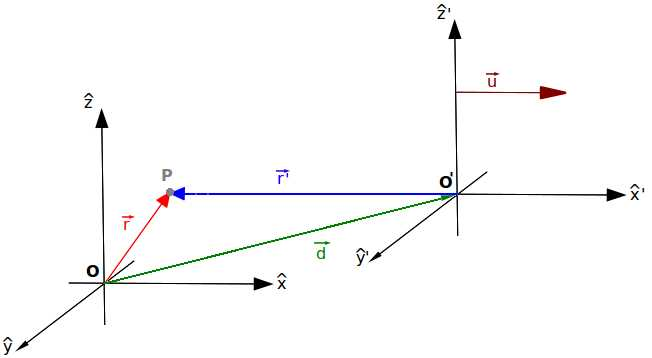
\includegraphics[scale=0.5]{immagini/galileo/sistemi}
  \caption{Cambio di coordinate tra sistemi inerziali.}
\end{figure}

Troviamo che valgono le seguenti leggi di trasformazione:
\begin{legge}
\begin{equation}\label{cambio_sis}
\ve r(t)=\overrightarrow{\left(O'-O\right)}+\ve r\,'= \ve d +\ve r = \ve u t+\ve r\,' 
\end{equation}
con $\ve d = \overrightarrow{\left(O'-O\right)} = \ve u t$ vettore di separazione tra i due sistemi.
\end{legge}
\begin{legge}[composizione delle velocità]
\index{composizione delle velocità}
\begin{equation}\label{cambio_vel}
\ve v=\frac{\ud\ve r}{\ud t}=\frac{\ud}{\ud t}\left(\ve u
t+\ve r\,'\right)=\frac{d}{\ud t}\left(\ve u
t\right)+\frac{\ud\ve r\,'}{\ud t}=\ve u+\frac{\ud\ve r\,'}{\ud
t'}=\ve u+\ve v\,' 
\end{equation}
usando la \ref{cambio_sis} si ottiene la \ref{cambio_vel}.
\end{legge}
\begin{legge}[invarianza dell'accelerazione]
\begin{equation}
\ve a=\frac{\ud \ve v}{\ud t}=\frac{\ud}{\ud t}(\ve u+\ve
v\,')=0+\frac{\ud \ve v\,'}{\ud t}=\frac{\ud \ve v\,'}{\ud
t'}=\ve a' 
\end{equation}
Concludiamo quindi che l'accelerazione è invariante: sistemi di riferimento diversi, ma inerziali misurano la stessa accelerazione 
per un corpo.
\end{legge}

Riassiumiano di seguito le trasformazioni di Galileo:
\begin{equation}\label{trasformazioni_galileo}
\left\{\begin{array}{ll}
\ve r=\ve r\,'+\ve u t&\\
\ve v=\ve u+\ve v\,'&\text{somma delle velocità}\\
\ve a=\ve a\,'&\text{invarianza dell'accelerazione}\\
t=t'&\text{ipotesi del tempo assoluto}\\
\end{array}\right. 
\end{equation}
In questo senso non esiste un sistema di riferimento privilegiato, ma le descrizione della fisica è equivalente in ogni sistema che si
muova di moto rettilineo uniforme (ovvero che sia inerziale) rispetto ad un altro. Il problema di questo approccio è il fatto che
è necessario assumere che esista almeno un sistema inerziale dal quale (con le trasformazioni di galieleo) si possano trovare tutti
gli altri. Questo sistema (il sistema ``fermo'') è quello delle stelle fisse.
\begin{Es}[lancio del sasso]
 Consideriamo due sistemi inerziali $O$ e $O'$. $O$ veda $O'$ muoversi lungo l'asse $x$ con velocità $\ve w$. Siano gli assi $y$ e $z$ uguali nei due sistemi. $O$ lancia un sasso verso l'alto, le equazioni del moto per il sasso visto da $O$ sono:
 \begin{gather*}
  x(t) = x_0\\
  y(t) = -\frac{1}{2}gt^2 + v_0 t
 \end{gather*}
 la traiettoria in questo caso è un segmento verticale con gli estremi in $(x_0,0)$ e $(x_0,\frac{v_0^2}{2g})$. Nel sistema $O'$ invece questo moto diventa:
 \begin{gather*}
  x'(t) = x(t) - w t = x_0 - wt\\
  y(t) = -\frac{1}{2}gt^2 + v_0 t
 \end{gather*}
 si noti che $v_0$ è sempre lo stesso nei due sistemi. Eliminando il tempo: $t = (x_0-x') /w$ si ottiene l'equazione di una parabola il cui vertice è ad una altezza uguale a quella nel sistema di $O$.
\end{Es}

\subsection{Rotazioni\index{rotazione}}

All'interno delle trasformazioni di Galileo possiamo annoverare anche le rotazioni.

In due dimensioni, una rotazione è una trasformazione $R(\theta)$, 
che dipende da un angolo $\theta$, e che trasforma il vettore $(x, y)$ in
\begin{equation}\label{rotazione}
\left\{\begin{array}{ll}
x'=x\cos\theta-y\sin\theta \\
y'=x\sin\theta+y\cos\theta
\end{array}\right. 
\end{equation}

Usando la moltiplicazione di matrici la rotazione può essere descritta così:
\begin{equation}
\begin{bmatrix} x' \\ y' \end{bmatrix} =
\begin{bmatrix} \cos \theta & -\sin \theta \\ \sin \theta & \cos \theta \end{bmatrix} 
\begin{bmatrix} x \\ y \end{bmatrix}
\end{equation}

La matrice quadrata presente in questa espressione è una matrice ortonormale di rango due. 
Questa trasformazione è chiamata ``rotazione antioraria'' di angolo $\theta$ intorno all'origine.
La matrice $2 \times 2$ che descrive la rotazione è spesso chiamata matrice di rotazione di angolo $\theta$

Se ora specializziamo la \ref{rotazione} per un angolo di $\theta = \frac{\pi}{6} = 30\degree$ abbiamo:
\begin{equation}\label{rotazione}
\left\{\begin{array}{ll}
x'=\dfrac{\sqrt{3}}{2}x-\dfrac{1}{2}y\\
y'=\dfrac{1}{2}x+\dfrac{\sqrt{3}}{2}y
\end{array}\right. 
\end{equation}
\begin{figure}[htbp]
  \centering
  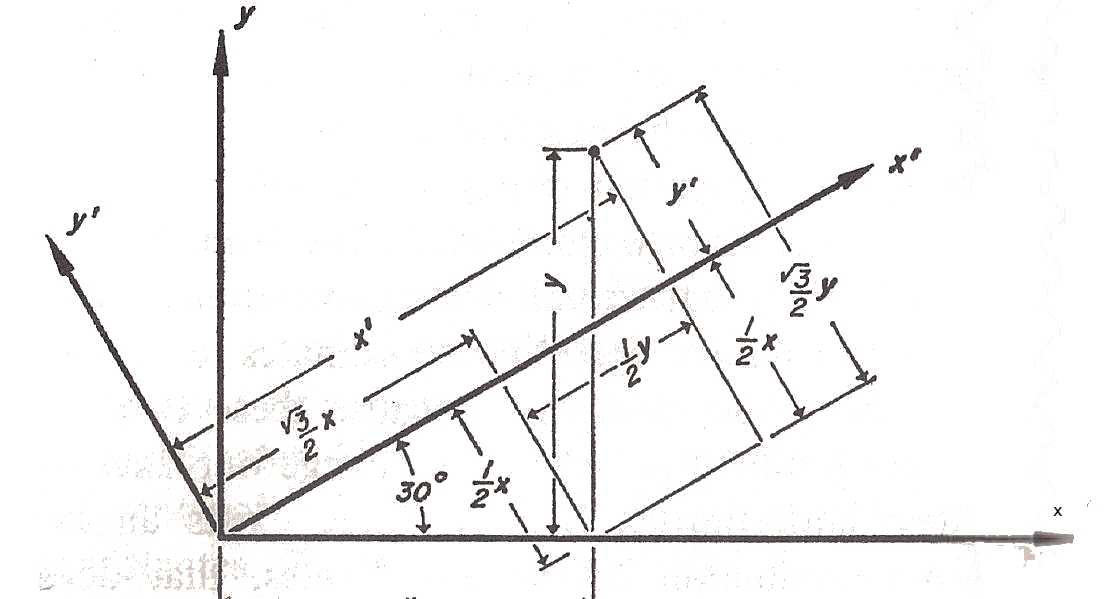
\includegraphics[scale=0.25]{immagini/galileo/rotaz}
  \caption{\label{Irotazionepi30}Una rotazione di $\dfrac{\pi}{3}$.}
\end{figure}

da confrontare con la figura \ref{Irotazionepi30}.

\section{Invarianza e covarianza\index{invarianza}\index{covarianza}}
Una grandezza si dice invariante se è numericamente uguale alla sua trasformata, cioè $x=T(x)=x'$.
Nelle trasformazioni di Galileo l'accelerazione è invariante rispetto alla trasformazione che trasforma le coordinate di $O$
in quelle di $O'$. Nella relatività galileiana la lunghezza è invariante, nella relatività ristretta no.

Una legge si dice covariante se la sua espressione è uguale alla sua trasformata, cioè $f(x)=T(f(x))$.

Concludiamo quindi che le leggi della dinamica ed in particolare la seconda legge di Newtown:
\begin{equation}\label{seconda_newton}
 \ve F = m \ve a 
\end{equation}
è invariante. Cioè, dato che tutti gli osservatori misureranno la stessa accelerazione $\ve a$, tutti concorderanno con 
\ref{seconda_newton}

Un altro esempio di oggetto invariante e che ci tornerà utile dopo è la distanza tra due punti quando si ruota o trasla 
il sistema di riferimento, abbiamo già visto com'è definita la distanza precedentemente.
Prendendo la distanza di un punto $P$ di coordinate $(x,y)$ indicato da un vettore $\ve P$, 
la sua distanza (al quadrato) dall'origine si scrive:
\begin{equation}\label{distanza_galileo}
 ||\ve P|| = x^2 + y^2 = s^2
\end{equation}

Se ruotiamo il sistema di riferimento abbiamo:
\begin{figure}[htbp]
  \centering
  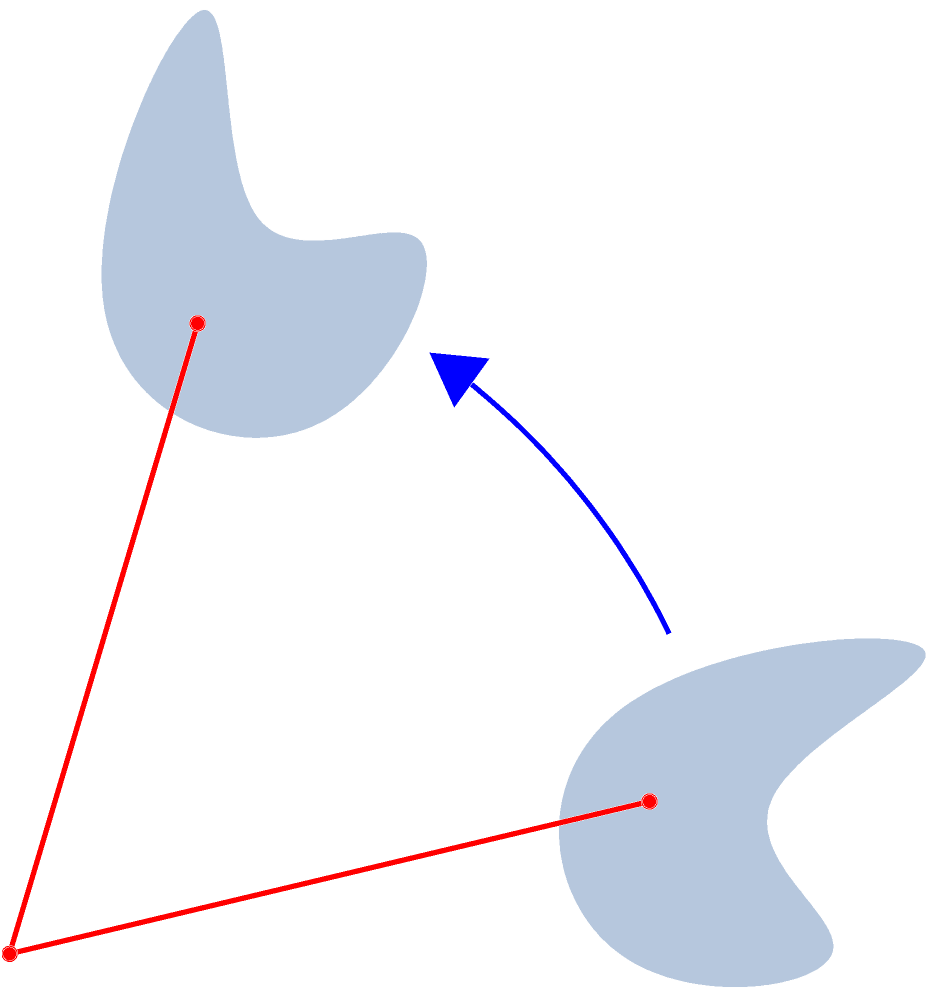
\includegraphics[scale=0.05]{immagini/galileo/Rotation_illustration}
  \caption{Rotazione antioraria nel piano.}
\end{figure}

Se sostituiamo \ref{rotazione} in \ref{distanza_galileo} abbiamo:
\begin{equation}
\begin{split}
s^2 &= {x'}^2 + {y'}^2 = \\
&= \left[\left(\dfrac{\sqrt{3}}{2}x-\dfrac{1}{2}y\right)^2 + \left(\dfrac{1}{2}x+\dfrac{\sqrt{3}}{2}y\right)^2\right] =\\
&= 4\dfrac{x^2 + y^2}{4} = x^2 +y^2
\end{split}
\end{equation}

e vediamo la quantità $s^2$ definita come sopra è invariante.